% Options for packages loaded elsewhere
\PassOptionsToPackage{unicode}{hyperref}
\PassOptionsToPackage{hyphens}{url}
%
\documentclass[
]{book}
\usepackage{amsmath,amssymb}
\usepackage{lmodern}
\usepackage{iftex}
\ifPDFTeX
  \usepackage[T1]{fontenc}
  \usepackage[utf8]{inputenc}
  \usepackage{textcomp} % provide euro and other symbols
\else % if luatex or xetex
  \usepackage{unicode-math}
  \defaultfontfeatures{Scale=MatchLowercase}
  \defaultfontfeatures[\rmfamily]{Ligatures=TeX,Scale=1}
\fi
% Use upquote if available, for straight quotes in verbatim environments
\IfFileExists{upquote.sty}{\usepackage{upquote}}{}
\IfFileExists{microtype.sty}{% use microtype if available
  \usepackage[]{microtype}
  \UseMicrotypeSet[protrusion]{basicmath} % disable protrusion for tt fonts
}{}
\makeatletter
\@ifundefined{KOMAClassName}{% if non-KOMA class
  \IfFileExists{parskip.sty}{%
    \usepackage{parskip}
  }{% else
    \setlength{\parindent}{0pt}
    \setlength{\parskip}{6pt plus 2pt minus 1pt}}
}{% if KOMA class
  \KOMAoptions{parskip=half}}
\makeatother
\usepackage{xcolor}
\IfFileExists{xurl.sty}{\usepackage{xurl}}{} % add URL line breaks if available
\IfFileExists{bookmark.sty}{\usepackage{bookmark}}{\usepackage{hyperref}}
\hypersetup{
  pdftitle={Excel for General Chemistry},
  pdfauthor={David Hall, David Liu, and Jessica D'eon},
  hidelinks,
  pdfcreator={LaTeX via pandoc}}
\urlstyle{same} % disable monospaced font for URLs
\usepackage{color}
\usepackage{fancyvrb}
\newcommand{\VerbBar}{|}
\newcommand{\VERB}{\Verb[commandchars=\\\{\}]}
\DefineVerbatimEnvironment{Highlighting}{Verbatim}{commandchars=\\\{\}}
% Add ',fontsize=\small' for more characters per line
\usepackage{framed}
\definecolor{shadecolor}{RGB}{248,248,248}
\newenvironment{Shaded}{\begin{snugshade}}{\end{snugshade}}
\newcommand{\AlertTok}[1]{\textcolor[rgb]{0.94,0.16,0.16}{#1}}
\newcommand{\AnnotationTok}[1]{\textcolor[rgb]{0.56,0.35,0.01}{\textbf{\textit{#1}}}}
\newcommand{\AttributeTok}[1]{\textcolor[rgb]{0.77,0.63,0.00}{#1}}
\newcommand{\BaseNTok}[1]{\textcolor[rgb]{0.00,0.00,0.81}{#1}}
\newcommand{\BuiltInTok}[1]{#1}
\newcommand{\CharTok}[1]{\textcolor[rgb]{0.31,0.60,0.02}{#1}}
\newcommand{\CommentTok}[1]{\textcolor[rgb]{0.56,0.35,0.01}{\textit{#1}}}
\newcommand{\CommentVarTok}[1]{\textcolor[rgb]{0.56,0.35,0.01}{\textbf{\textit{#1}}}}
\newcommand{\ConstantTok}[1]{\textcolor[rgb]{0.00,0.00,0.00}{#1}}
\newcommand{\ControlFlowTok}[1]{\textcolor[rgb]{0.13,0.29,0.53}{\textbf{#1}}}
\newcommand{\DataTypeTok}[1]{\textcolor[rgb]{0.13,0.29,0.53}{#1}}
\newcommand{\DecValTok}[1]{\textcolor[rgb]{0.00,0.00,0.81}{#1}}
\newcommand{\DocumentationTok}[1]{\textcolor[rgb]{0.56,0.35,0.01}{\textbf{\textit{#1}}}}
\newcommand{\ErrorTok}[1]{\textcolor[rgb]{0.64,0.00,0.00}{\textbf{#1}}}
\newcommand{\ExtensionTok}[1]{#1}
\newcommand{\FloatTok}[1]{\textcolor[rgb]{0.00,0.00,0.81}{#1}}
\newcommand{\FunctionTok}[1]{\textcolor[rgb]{0.00,0.00,0.00}{#1}}
\newcommand{\ImportTok}[1]{#1}
\newcommand{\InformationTok}[1]{\textcolor[rgb]{0.56,0.35,0.01}{\textbf{\textit{#1}}}}
\newcommand{\KeywordTok}[1]{\textcolor[rgb]{0.13,0.29,0.53}{\textbf{#1}}}
\newcommand{\NormalTok}[1]{#1}
\newcommand{\OperatorTok}[1]{\textcolor[rgb]{0.81,0.36,0.00}{\textbf{#1}}}
\newcommand{\OtherTok}[1]{\textcolor[rgb]{0.56,0.35,0.01}{#1}}
\newcommand{\PreprocessorTok}[1]{\textcolor[rgb]{0.56,0.35,0.01}{\textit{#1}}}
\newcommand{\RegionMarkerTok}[1]{#1}
\newcommand{\SpecialCharTok}[1]{\textcolor[rgb]{0.00,0.00,0.00}{#1}}
\newcommand{\SpecialStringTok}[1]{\textcolor[rgb]{0.31,0.60,0.02}{#1}}
\newcommand{\StringTok}[1]{\textcolor[rgb]{0.31,0.60,0.02}{#1}}
\newcommand{\VariableTok}[1]{\textcolor[rgb]{0.00,0.00,0.00}{#1}}
\newcommand{\VerbatimStringTok}[1]{\textcolor[rgb]{0.31,0.60,0.02}{#1}}
\newcommand{\WarningTok}[1]{\textcolor[rgb]{0.56,0.35,0.01}{\textbf{\textit{#1}}}}
\usepackage{longtable,booktabs,array}
\usepackage{calc} % for calculating minipage widths
% Correct order of tables after \paragraph or \subparagraph
\usepackage{etoolbox}
\makeatletter
\patchcmd\longtable{\par}{\if@noskipsec\mbox{}\fi\par}{}{}
\makeatother
% Allow footnotes in longtable head/foot
\IfFileExists{footnotehyper.sty}{\usepackage{footnotehyper}}{\usepackage{footnote}}
\makesavenoteenv{longtable}
\usepackage{graphicx}
\makeatletter
\def\maxwidth{\ifdim\Gin@nat@width>\linewidth\linewidth\else\Gin@nat@width\fi}
\def\maxheight{\ifdim\Gin@nat@height>\textheight\textheight\else\Gin@nat@height\fi}
\makeatother
% Scale images if necessary, so that they will not overflow the page
% margins by default, and it is still possible to overwrite the defaults
% using explicit options in \includegraphics[width, height, ...]{}
\setkeys{Gin}{width=\maxwidth,height=\maxheight,keepaspectratio}
% Set default figure placement to htbp
\makeatletter
\def\fps@figure{htbp}
\makeatother
\setlength{\emergencystretch}{3em} % prevent overfull lines
\providecommand{\tightlist}{%
  \setlength{\itemsep}{0pt}\setlength{\parskip}{0pt}}
\setcounter{secnumdepth}{5}
\usepackage{booktabs}
\usepackage{amsthm}
\makeatletter
\def\thm@space@setup{%
  \thm@preskip=8pt plus 2pt minus 4pt
  \thm@postskip=\thm@preskip
}
\makeatother
\ifLuaTeX
  \usepackage{selnolig}  % disable illegal ligatures
\fi
\usepackage[]{natbib}
\bibliographystyle{plainnat}

\title{Excel for General Chemistry}
\author{David Hall, David Liu, and Jessica D'eon}
\date{Book last built on 2022-06-10}

\begin{document}
\maketitle

{
\setcounter{tocdepth}{1}
\tableofcontents
}
\hypertarget{preface}{%
\chapter*{Preface}\label{preface}}
\addcontentsline{toc}{chapter}{Preface}

Placeholder

\hypertarget{providing-feedback}{%
\section*{Providing Feedback}\label{providing-feedback}}
\addcontentsline{toc}{section}{Providing Feedback}

\hypertarget{authors}{%
\section*{Authors}\label{authors}}
\addcontentsline{toc}{section}{Authors}

\hypertarget{acknowlegements}{%
\section*{Acknowlegements}\label{acknowlegements}}
\addcontentsline{toc}{section}{Acknowlegements}

\hypertarget{intro}{%
\chapter{Introduction}\label{intro}}

Placeholder

\hypertarget{ozone-is-not-our-friend}{%
\section{Ozone is Not Our Friend}\label{ozone-is-not-our-friend}}

\hypertarget{atmospheric-concentration-units}{%
\section{Atmospheric Concentration Units}\label{atmospheric-concentration-units}}

\hypertarget{capabilities}{%
\chapter{Getting Setup for Success}\label{capabilities}}

Placeholder

\hypertarget{accessing-the-microsoft-office-suite-of-software}{%
\section{Accessing the Microsoft Office Suite of Software}\label{accessing-the-microsoft-office-suite-of-software}}

\hypertarget{managing-your-files}{%
\section{Managing your Files}\label{managing-your-files}}

\hypertarget{creating-professional-documents}{%
\section{Creating Professional Documents}\label{creating-professional-documents}}

\hypertarget{adding-an-excel-graph-into-a-word-document}{%
\subsection{Adding an Excel Graph into a Word Document}\label{adding-an-excel-graph-into-a-word-document}}

\hypertarget{creating-a-pdf-from-a-word-document}{%
\subsection{Creating a PDF from a Word Document}\label{creating-a-pdf-from-a-word-document}}

\hypertarget{data-wrangling}{%
\chapter{Data Wrangling}\label{data-wrangling}}

Placeholder

\hypertarget{file-upload}{%
\section{File Upload}\label{file-upload}}

\hypertarget{data-organization-and-cell-formatting}{%
\section{Data Organization and Cell Formatting}\label{data-organization-and-cell-formatting}}

\hypertarget{data-manipulation}{%
\section{Data Manipulation}\label{data-manipulation}}

\hypertarget{math-stats-and-programming}{%
\chapter{Math, Stats, and Programming}\label{math-stats-and-programming}}

Physical chemistry is a quantitative science, meaning we use mathematical operations to explain and explore chemical phenomena. This math can be done by hand, but once you have more than one or two data points this gets very tiring and a spreadsheet can be a lifesaver! In this section we will talk about how to program mathematical equations into Excel, how to use common mathematical and statistical functions, and how to reference other values within the spreadsheet. We will also dip our toes into some simple computer programming that can be very useful.

\hypertarget{mathematical-operations}{%
\section{Mathematical Operations}\label{mathematical-operations}}

Excel can perform many mathematical operations and the table below provides a list of some of the most common common operations with their corresponding formula.

\begin{longtable}[]{@{}
  >{\raggedright\arraybackslash}p{(\columnwidth - 8\tabcolsep) * \real{0.1908}}
  >{\raggedright\arraybackslash}p{(\columnwidth - 8\tabcolsep) * \real{0.4733}}
  >{\raggedright\arraybackslash}p{(\columnwidth - 8\tabcolsep) * \real{0.1603}}
  >{\raggedright\arraybackslash}p{(\columnwidth - 8\tabcolsep) * \real{0.1527}}
  >{\raggedright\arraybackslash}p{(\columnwidth - 8\tabcolsep) * \real{0.0229}}@{}}
\toprule
\begin{minipage}[b]{\linewidth}\raggedright
Input
\end{minipage} & \begin{minipage}[b]{\linewidth}\raggedright
Operator
\end{minipage} & \begin{minipage}[b]{\linewidth}\raggedright
Example\ldots{}
\end{minipage} & \begin{minipage}[b]{\linewidth}\raggedright
\ldots{} solves to
\end{minipage} & \begin{minipage}[b]{\linewidth}\raggedright
\end{minipage} \\
\midrule
\endhead
= & Equal sign indicates a mathematical operation & & & \\
+ & Addition & =2+2 & 4 & \\
- & Subtraction & =3--2 & 1 & \\
* & Multiplication & =3*2 & 6 & \\
/ & Division & =4/2 & 2 & \\
\^{} & Exponent & =4\^{}2 & 16 & \\
( ) & Brackets to indicate order of operations & =(4+2)*2 & 12 & \\
LOG(number,base) & Logarithm (10 is the default if no base is indicated) & =LOG(100,10) & 2 & \\
LN(number) & Natural Logarithm & =LN(2) & 0.693\ldots{} & \\
\bottomrule
\end{longtable}

Recall chemical equations (\ref{eq1}) to (\ref{eq3}) from the \protect\hyperlink{intro}{Introduction} that describe the relationship between NO\textsubscript{2} and O\textsubscript{3}.

\[
\begin{align}
    NO_2 + h\nu → NO + O && \label{eq1}\tag{1} \\
O + O_2 →  O_3 &&  \label{eq2}\tag{2}  \\
    O_3 + NO →  O_2 + NO_2 &&  \label{eq3}\tag{3}
\end{align}
\]
Also, recall that because these two pollutants are so intimately linked atmospheric chemists have defined a term called ``odd oxygen'' or O\textsubscript{X} that is the sum of NO\textsubscript{2} and O\textsubscript{3} at a given time point.

\[
\begin{align}
    [O_3] + [NO_2] &= [O_X] \label{eq4}\tag{4} 
\end{align}
\]

To add O\textsubscript{X} to your analysis you will need to calculate the concentration O\textsubscript{X} at each timepoint in your dataset. You can do this by simply adding the cells containing O\textsubscript{3} and NO\textsubscript{2} (both concentrations are in ppb so they can be added directly) for the first timepoint then copy this formula down the column. When you add a formula into Excel remember to start with a ``='' sign (this will let Excel know you are writing a formula), if you are referencing a cell you can either write it in (e.g.~``C2'') or you can click on the cell. Once your formula is complete, hit ENTER and Excel will perform the calculation.

To copy the formula from one cell down the list of data points, you can use the copy and paste function in the edit menu or the keyboard shortcuts, CONTROL+C to copy and CONTROL+V to pasta (COMMAND+C and COMMAND+V on Mac) to copy the formula. You can also use a shortcut specific to Excel. Click on the cell with your formula and notice the little square in the lower righthand corner. Click on this square and drag the formula down the column, or, even better, double click on the square and Excel will automatically paste the formula down the column until the end of the series (note that it will stop at the first blank cell so if you are missing values you may need to copy and paste the formula the rest of the way). When you add a new value, make sure you remember to label your column.

\begin{Shaded}
\begin{Highlighting}[]
\NormalTok{knitr}\SpecialCharTok{::}\FunctionTok{include\_graphics}\NormalTok{(}\AttributeTok{path=}\StringTok{"./gifs/OxCalc.gif"}\NormalTok{)}
\end{Highlighting}
\end{Shaded}

\includegraphics{./gifs/OxCalc.gif}

If you are learning about mathematical operations in Excel for the first time we strongly suggest reading the next section on cell referencing.

\hypertarget{cell-referencing}{%
\section{Cell Referencing}\label{cell-referencing}}

One of Excel's strengths is its ability to easily perform mathematical operations in larger datasets. To take advantage of this feature it is important to appreciate how Excel references values in the spreadsheet. Simply referencing a cell in Excel will add a relative reference, which means that the reference will move as the equation is copied and pasted to other cells. This is the type of reference created in the O\textsubscript{X} calculation in the section above. If you are unsure of the cells being referenced in an equation Excel will visualize the reference when you click on the cell.

\begin{Shaded}
\begin{Highlighting}[]
\NormalTok{knitr}\SpecialCharTok{::}\FunctionTok{include\_graphics}\NormalTok{(}\AttributeTok{path=}\StringTok{"./gifs/RelRef.gif"}\NormalTok{)}
\end{Highlighting}
\end{Shaded}

\includegraphics{./gifs/RelRef.gif}

A relative reference is very useful when calculating a series of numbers, like O\textsubscript{X} from O\textsubscript{3} and NO\textsubscript{2}, however there are times when you might wish to make a reference absolute, such that it does not move as it is copied and pasted. To do this you add a \$ in front of the letter and/or the number in the cell reference. It is possible to add a \$ to only the letter (column reference) or the number (row reference) and only lock one aspect of the referencing or to lock both.

The gif below, which is a spreadsheet setup to calculate the energy of a photon in J/molecule from its wavelength in nm, is an example that includes both absolute and relative references. The equation to calculate energy includes absolute references to the relevant constants and a relative reference to the wavelength of the photon such that is moves as the equation is copied down the column. As shown in the gif, if the absolute reference is not properly applied the calculated values don't make any sense.

\begin{Shaded}
\begin{Highlighting}[]
\NormalTok{knitr}\SpecialCharTok{::}\FunctionTok{include\_graphics}\NormalTok{(}\AttributeTok{path=}\StringTok{"./gifs/EnergyCalc.gif"}\NormalTok{)}
\end{Highlighting}
\end{Shaded}

\includegraphics{./gifs/EnergyCalc.gif}

\hypertarget{simple-statistical-functions}{%
\section{Simple Statistical Functions}\label{simple-statistical-functions}}

When we have a several measurements it is often useful to know how they compare to one another. To get a sense of that we can employ some simple statistical functions. One such function is a mean or average value, given the symbol \(\overline{x}\). Another typical function is a standard deviation, given the symbol \(\sigma\). We typically understand what a mean value represents, but what is a standard deviation? The mathematical formula for the standard deviation of a set of samples is shown in equation 9:

\[ \begin{align}
\sum \frac{\left(x-\overline{x}\right)^{2}}{N-1} \label{eq9}\tag{9} 
\end{align} \]

where \(\x_i\) is the individual data points within the dataset; \(\overline{x}\) is the mean value of the dataset; and N is the number of values in the dataset. Looking at this formula it is clear that standard deviation is related to the difference between the individual values in the dataset and the mean value of the dataset. Standard deviation is a useful metric for appreciating the spread in the data. The greater the spread, the greater the standard deviation. More specifically, as shown in the figure below, one standard deviation away from the mean on either side will include 68\% of the data points and two standard deviations will include 95\% of the data.

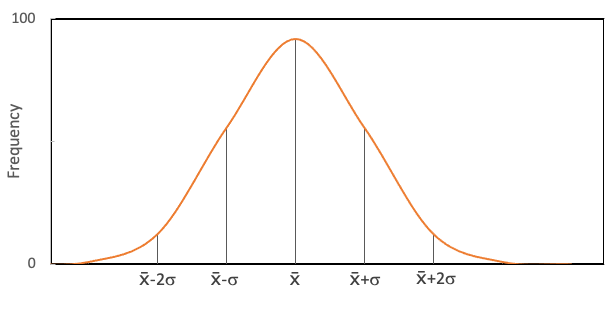
\includegraphics{images/StandardDeviation.png}

Standard deviation is a useful metric, however the magnitude of the spread in the data is often related to the overall magnitude of the values. For example, the standard deviation of 0.5 is large for a dataset with a mean value of 1, but small for a dataset with a mean value of 50. To provide this context we can calculate a relative standard deviation (RSD), which is calculated by dividing the standard deviation by the mean value and then multiplying this ratio by 100 (equation \ref{eq10}).

\[ 
\begin{align}
RSD = \frac{\sigma}{\overline{x}} \times 100 \label{eq10}\tag{10} 
\end{align}
\]

The RSD of a dataset expresses the magnitude of the spread in the data using a percentage to normalize for differences in magnitude (e.g.~a dataset with a mean value of 1 and a standard deviation of 0.5 has an RSD of 50\%, and that with a mean value of 50 and a standard deviation of 0.5 has an RSD of 1\%).

The table below presents formula and descriptions to calculate the mean, median, standard deviation, as well as the minimum and maximum values for a set of numbers.

\begin{longtable}[]{@{}
  >{\raggedright\arraybackslash}p{(\columnwidth - 8\tabcolsep) * \real{0.2523}}
  >{\raggedright\arraybackslash}p{(\columnwidth - 8\tabcolsep) * \real{0.2890}}
  >{\raggedright\arraybackslash}p{(\columnwidth - 8\tabcolsep) * \real{0.4312}}
  >{\raggedright\arraybackslash}p{(\columnwidth - 8\tabcolsep) * \real{0.0138}}
  >{\raggedright\arraybackslash}p{(\columnwidth - 8\tabcolsep) * \real{0.0138}}@{}}
\toprule
\begin{minipage}[b]{\linewidth}\raggedright
Calculation
\end{minipage} & \begin{minipage}[b]{\linewidth}\raggedright
Formula
\end{minipage} & \begin{minipage}[b]{\linewidth}\raggedright
Description
\end{minipage} & \begin{minipage}[b]{\linewidth}\raggedright
\end{minipage} & \begin{minipage}[b]{\linewidth}\raggedright
\end{minipage} \\
\midrule
\endhead
Mean & =AVERAGE(number1, {[}number2{]}, \ldots) & Returns the arithmetic mean of the inputs. & & \\
Median & =MEDIAN(number1, {[}number2{]}, \ldots) & Returns the middle number in a group of supplied number. & & \\
Standard Deviation (recommended for Experiment 1) & =STDEV.S(number1, {[}number2{]}, \ldots) =STDEV(number1, {[}number2{]}, \ldots) & Returns the standard deviation of the samples provided (the two equations are equivalent). & & \\
Standard Deviation (not recommended for Experiment 1) & =STDEV.P(number1, {[}number2{]}, \ldots) & Returns the standard deviation assuming that the samples provided are the entire population. & & \\
Minimum & =MIN(number1, {[}number2{]}, \ldots) & Returns the minimum value in a set of numbers. & & \\
Maximum & =MAX(number1, {[}number2{]}, \ldots) & Returns the maximum value in a set of numbers. & & \\
\bottomrule
\end{longtable}

The figure below provides some context on how to use these formulas with an example calculating the mean, median, standard deviation, relative standard deviation, minimum and maximum values of a list of outdoor summer temperatures in Toronto. The formula for each calculation is provided as text next to the value in question (note the quotation marks). Keep in mind that Excel will help you with these calculations, once you put an equal sign into the equation bar and start typing it will give you suggestions of possible functions, don't be afraid to use them. Once you select the function and the brackets are open you can also select one cell, or a series of cells, using the cursor as opposed to writing them in.

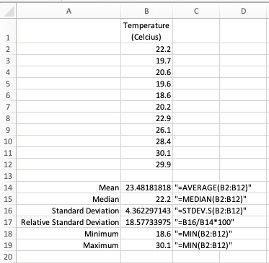
\includegraphics{images/SimpleStats.png}

\hypertarget{useful-functions-and-simple-programming}{%
\section{Useful Functions and Simple Programming}\label{useful-functions-and-simple-programming}}

details on if statements
details on calculating the slope and intercept in the excel spreadsheet

\hypertarget{troubleshooting}{%
\section{Troubleshooting}\label{troubleshooting}}

maybe some notes on common errors and how to approach troubleshooting
might be useful to mention what an \#N/A is and div0

\hypertarget{data-visualization}{%
\chapter{Data Visualization}\label{data-visualization}}

Placeholder

\hypertarget{creating-a-scatterplot}{%
\section{Creating a Scatterplot}\label{creating-a-scatterplot}}

\hypertarget{including-plots}{%
\section{Including Plots}\label{including-plots}}

\hypertarget{bookdown-capabilities}{%
\chapter{Bookdown Capabilities}\label{bookdown-capabilities}}

Placeholder

\hypertarget{interactive-and-exportable-tables}{%
\section{Interactive and exportable tables}\label{interactive-and-exportable-tables}}

\hypertarget{animated-gifs}{%
\section{Animated GIFS}\label{animated-gifs}}

\hypertarget{embedded-videos}{%
\section{Embedded videos}\label{embedded-videos}}

\hypertarget{jessica-test-woo-hoo}{%
\section{Jessica Test, Woo hoo!}\label{jessica-test-woo-hoo}}

  \bibliography{book.bib,packages.bib}

\end{document}
